%
%  untitled 2
%
%  Created by Stephan Gabler on 2010-05-14.
%  Copyright (c) 2010 __MyCompanyName__. All rights reserved.
%
\documentclass[]{article}

% Use utf-8 encoding for foreign characters
\usepackage[utf8]{inputenc}

% Setup for fullpage use
\usepackage{fullpage}

% Uncomment some of the following if you use the features
%
% Running Headers and footers
%\usepackage{fancyhdr}

% Multipart figures
%\usepackage{subfigure}

% More symbols
%\usepackage{amsmath}
%\usepackage{amssymb}
%\usepackage{latexsym}

% Surround parts of graphics with box
\usepackage{boxedminipage}

% Package for including code in the document
\usepackage{listings}

% If you want to generate a toc for each chapter (use with book)
\usepackage{minitoc}

% This is now the recommended way for checking for PDFLaTeX:
\usepackage{ifpdf}

%\newif\ifpdf
%\ifx\pdfoutput\undefined
%\pdffalse % we are not running PDFLaTeX
%\else
%\pdfoutput=1 % we are running PDFLaTeX
%\pdftrue
%\fi

\ifpdf
\usepackage[pdftex]{graphicx}
\else
\usepackage{graphicx}
\fi
\title{Exercise 3, Machine Intelligence II}
\author{Group 1}

\date{\today}

\begin{document}

\ifpdf
\DeclareGraphicsExtensions{.pdf, .jpg, .tif}
\else
\DeclareGraphicsExtensions{.eps, .jpg}
\fi

\maketitle

\section{Comments} % (fold)
\label{sg:sec:comments}

Our task was to approximate/estimate the probability distribution of pixel
values in an image, given the assumption that the pixels are iid distributed.
Therefore we draw a sample from the image and compute its histogram which is
afterwards smoothed by a gaussian kernel of a certain width h. This can be
done by summation of gaussian kernels (each centered on a pixel value) or
by a convolution of the histogram with the kernel. We chose the first method
because we had some problems with the right indexing when we used the convolution
variant. In both cases the resulting function has to be normalized in order
to become a distribution. The optimal kernel width h which gives the best
estimate of the original distribution (evaluated on the pixels not used for
the estimation) is then determined by measuring the log-likelihood of this parameter. 

In 3 out of 4 cases the kernel with width h = 10 gave the best result
with respect to the likelihood. 


% section comments (end)

\section{Results}

\begin{figure}[ht]
	\centering
		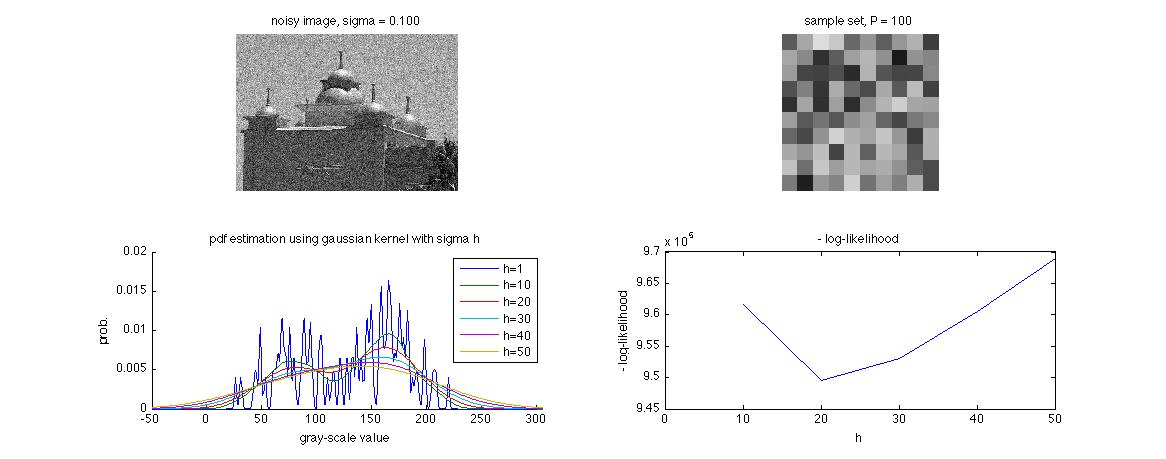
\includegraphics[width=0.8\textwidth]{plot100_01.jpg}
	\caption{P = 100, sigma = 0.1}
	\label{sg:fig:plot100_01}
\end{figure}

\begin{figure}[ht]
	\centering
		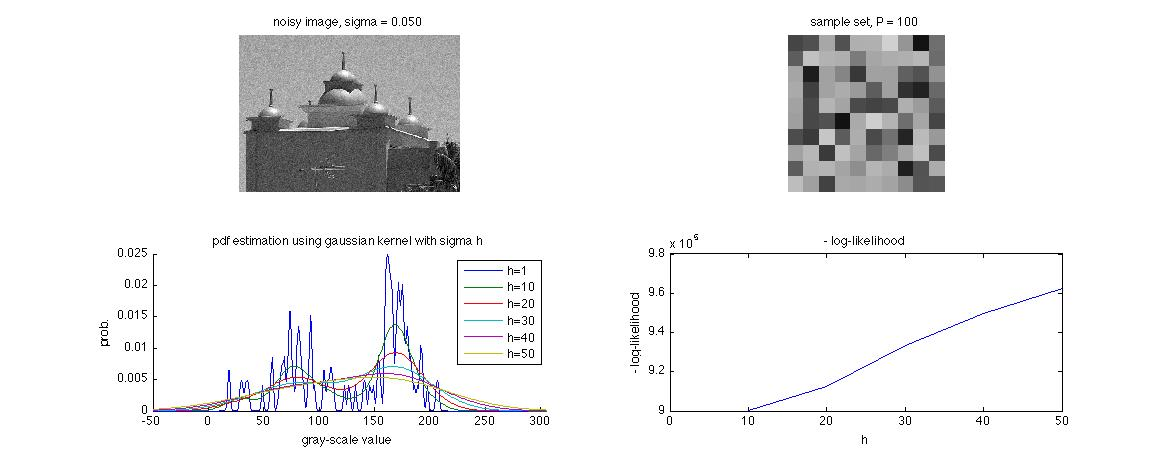
\includegraphics[width=0.8\textwidth]{plot100_005.jpg}
		\caption{P = 100, sigma = 0.05}
	\label{sg:fig:plot100_005}
\end{figure}

\begin{figure}[ht]
	\centering
		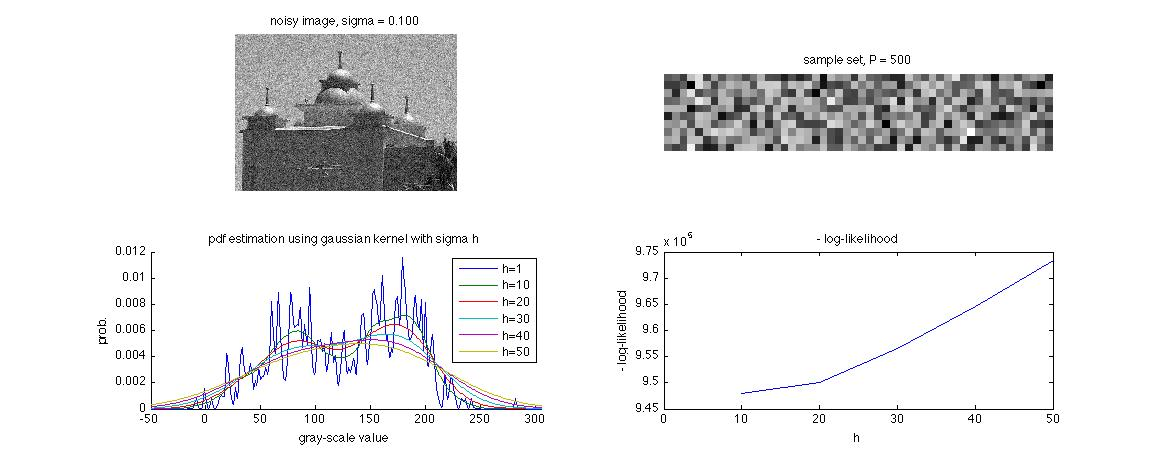
\includegraphics[width=0.8\textwidth]{plot500_01.jpg}
		\caption{P = 500, sigma = 0.1}
	\label{sg:fig:plot500_01}
\end{figure}

\begin{figure}[ht]
	\centering
		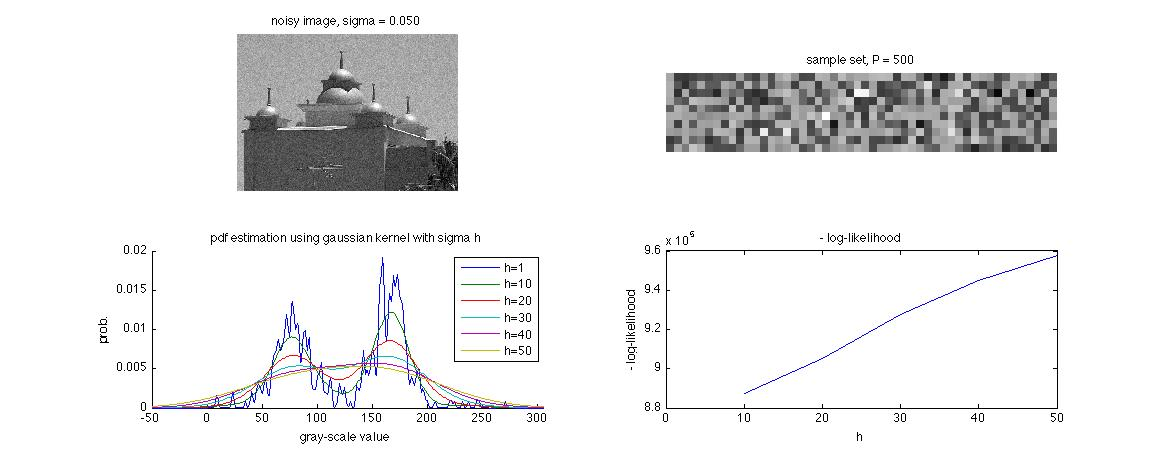
\includegraphics[width=0.8\textwidth]{plot500_005.jpg}
		\caption{P = 500, sigma = 0.05}
	\label{sg:fig:plot500_005}
\end{figure}

\begin{figure}[ht]
	\centering
		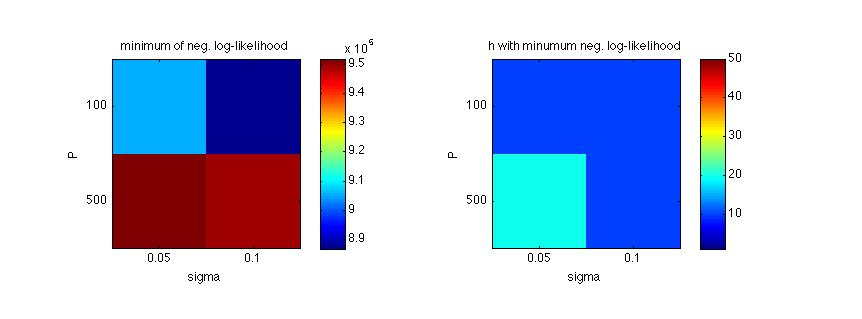
\includegraphics[width=0.8\textwidth]{best_log.jpg}
	\caption{The plot on the left shows the value of the negative log-likelihood 
	for different sigmas and sample sizes. While on the right its shown the value 
	of h which minimizes the negative log-likelihood for all the combinations of 
	sigmas and sample size, which appears to be h=10 for all.}
	\label{sg:fig:best_log}
\end{figure}


\end{document}
